% =========================================================
% Beamer Presentation: Sour Gas Sweetening for TA-58
% =========================================================

\documentclass[aspectratio=169, 11pt]{beamer}

% ============================================
% Packages
% ============================================
\usepackage{fontspec}
\usepackage{unicode-math}
\usepackage{amsmath}
\usepackage{siunitx}
\sisetup{detect-all, per-mode=symbol}
\DeclareSIUnit\USD{\$}
\DeclareSIUnit\yr{yr}
\DeclareSIUnit\ton{ton}

\usepackage[version=4]{mhchem}
\usepackage{booktabs}
\usepackage{tabularx}
\usepackage{graphicx}
\usepackage{adjustbox}

% TikZ
\usepackage{tikz}
\usetikzlibrary{
    positioning,
    arrows,
    arrows.meta,
    shapes,
    shapes.geometric,
    calc,
    decorations.pathmorphing,
    fit,
    backgrounds,
    mindmap,
    shadows
}

% ============================================
% Fonts
% ============================================
\setmainfont{STIX Two Text}
\setsansfont{TeX Gyre Heros}[Scale=0.95]
\setmonofont{TeX Gyre Cursor}[Scale=0.9]
\setmathfont{STIX Two Math}

% ============================================
% Theme
% ============================================
\usepackage{beamerthemestaatsolie}

% Define colors for TikZ (needed for graphics)
\definecolor{MainBlue}{RGB}{0,92,184}
\definecolor{AccentA}{RGB}{33,97,140}
\definecolor{AccentB}{RGB}{20,111,124}
\definecolor{AccentC}{RGB}{123,36,28}
\definecolor{Charcoal}{RGB}{60,60,60}
\definecolor{StageInk}{RGB}{15,15,15}
\definecolor{HintGray}{RGB}{95,95,95}

% TikZ styles (from report)
\tikzset{
    stage/.style={font=\bfseries\footnotesize, text=StageInk, align=center},
    hint/.style={font=\scriptsize, text=HintGray, align=center, inner sep=0pt},
    mainarrow/.style={->, line width=0.9pt, draw=MainBlue, >={Stealth[length=2mm,width=1.2mm]}},
    sidearrow/.style={->, line width=0.6pt, draw=Charcoal, >={Stealth[length=2mm,width=1.2mm]}},
    stepnum/.style={circle, inner sep=0pt, minimum size=4mm, font=\scriptsize\bfseries},
    stepmain/.style={stepnum, fill=MainBlue, text=white},
    stepside/.style={stepnum, fill=Charcoal, text=white}
}

% Graphics path
\graphicspath{{../Graphics/}}

% ============================================
% Metadata
% ============================================
\title{Sour Gas Sweetening for TA-58}
\subtitle{Conceptual Design Study --- SCT Technology Recommendation}
\author{Guillian Kasandikromo}
\institute{Process Engineering, P\&ES \\ Staatsolie Maatschappij Suriname N.V.}
\date{\today}

% ============================================
% Document
% ============================================
\begin{document}

% ============================================
% SLIDE 1: Title
% ============================================
\begin{frame}
    \maketitle
    \begin{tikzpicture}[remember picture, overlay]
        \node[anchor=south east, opacity=0.9] at (current page.south east) {
            \includegraphics[width=3cm]{Zwart Staatsolie logo - RGB.png}
        };
    \end{tikzpicture}
\end{frame}

% ============================================
% SLIDE 2: Project Context
% ============================================
\begin{frame}{Project Context}
    \begin{columns}[T]
        \begin{column}{0.45\textwidth}
            \textbf{The Opportunity}
            \begin{itemize}
                \item TA-58 flares sour associated gas
                \item Two Caterpillar G3408 engines run on diesel
                \item Diesel cost: \highlight{\$500,000/yr}
            \end{itemize}

            \vspace{0.5em}
            \textbf{The Challenge}
            \begin{itemize}
                \item Gas contains \SI{1800}{ppmv} \ce{H2S}
                \item Engine spec: $<$\SI{45}{ppmv} \ce{H2S}
                \item Need 97.5\% removal efficiency
            \end{itemize}
        \end{column}
        \begin{column}{0.55\textwidth}
            \centering
            \resizebox{0.95\textwidth}{!}{%
                % Design mindmap embedded directly
                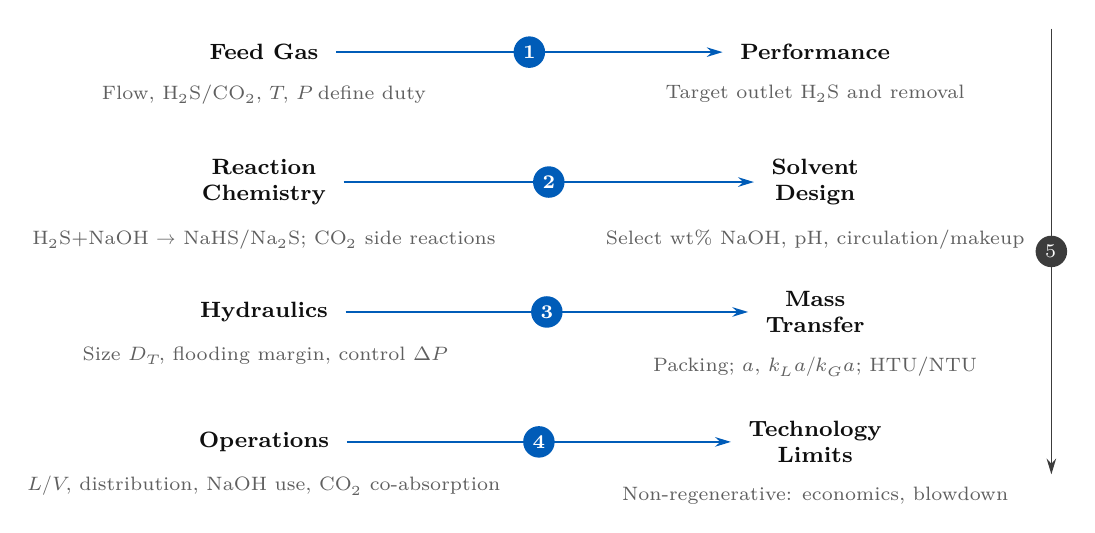
\begin{tikzpicture}[node distance=11mm and 36mm]
                    \coordinate (ColL) at (0,0);
                    \coordinate (ColR) at (7.0,0);
                    \coordinate (LaneX) at (10.0,0);
                    \def\RowGap{1.65}
                    \draw[sidearrow] ($(LaneX)+(0,0.3)$) -- node[stepside,pos=0.5]{$5$}($(LaneX)+(0,-3.25*\RowGap)$);
                    \node[stage] (feed) at (ColL) {Feed Gas};
                    \node[stage] (perf) at (ColR) {Performance};
                    \node[hint] [below=1.8mm of feed] {Flow, H$_2$S/CO$_2$, $T$, $P$ define duty};
                    \node[hint] [below=1.8mm of perf] {Target outlet H$_2$S and removal};
                    \draw[mainarrow] ([xshift=1mm]feed.east) -- node[stepmain, pos=0.5]{1} ([xshift=-1mm]perf.west);
                    \node[stage] (chem) at ($(ColL)+(0,-\RowGap)$) {Reaction\\Chemistry};
                    \node[stage] (solv) at ($(ColR)+(0,-\RowGap)$) {Solvent\\Design};
                    \node[hint] [below=1.8mm of chem] {H$_2$S+NaOH $\rightarrow$ NaHS/Na$_2$S; CO$_2$ side reactions};
                    \node[hint] [below=1.8mm of solv] {Select wt\% NaOH, pH, circulation/makeup};
                    \draw[mainarrow] ([xshift=1mm]chem.east) -- node[stepmain, pos=0.5]{2} ([xshift=-1mm]solv.west);
                    \node[stage] (hyd) at ($(ColL)+(0,-2*\RowGap)$) {Hydraulics};
                    \node[stage] (mt) at ($(ColR)+(0,-2*\RowGap)$) {Mass\\Transfer};
                    \node[hint] [below=1.8mm of hyd] {Size $D_T$, flooding margin, control $\Delta P$};
                    \node[hint] [below=1.8mm of mt] {Packing; $a$, $k_La/k_Ga$; HTU/NTU};
                    \draw[mainarrow] ([xshift=1mm]hyd.east) -- node[stepmain, pos=0.5]{3} ([xshift=-1mm]mt.west);
                    \node[stage] (ops) at ($(ColL)+(0,-3*\RowGap)$) {Operations};
                    \node[stage] (lim) at ($(ColR)+(0,-3*\RowGap)$) {Technology\\Limits};
                    \node[hint] [below=1.8mm of ops] {$L/V$, distribution, NaOH use, CO$_2$ co-absorption};
                    \node[hint] [below=1.8mm of lim] {Non-regenerative: economics, blowdown};
                    \draw[mainarrow] ([xshift=1mm]ops.east) -- node[stepmain, pos=0.5]{4} ([xshift=-1mm]lim.west);
                \end{tikzpicture}
            }
        \end{column}
    \end{columns}
\end{frame}

% ============================================
% SLIDE 3: Feed Characterization
% ============================================
\begin{frame}{Design Basis}
    \begin{columns}[c]
        \begin{column}{0.5\textwidth}
            \centering
            \begin{tabular}{@{}lc@{}}
                \toprule
                \textbf{Parameter} & \textbf{Value} \\
                \midrule
                Flow rate & \textbf{660,000 SCFD} \\
                Molar flow & 31.3 kmol/h \\
                Inlet \ce{H2S} & 1,800 ppmv \\
                Inlet \ce{CO2} & 28,550 ppmv \\
                Target \ce{H2S} & $<$45 ppmv \\
                Temperature & 25--40 °C \\
                Pressure & Atmospheric \\
                \bottomrule
            \end{tabular}
        \end{column}
        \begin{column}{0.5\textwidth}
            \textbf{Component Flows}
            \vspace{0.5em}

            \begin{tabular}{@{}lcc@{}}
                \toprule
                & \textbf{kmol/h} & \textbf{kg/day} \\
                \midrule
                \ce{H2S} & 0.056 & 46 \\
                \ce{CO2} & 0.90 & 950 \\
                \bottomrule
            \end{tabular}

            \vspace{1em}
            \centering
            \Large
            \textcolor{AccentC}{\textbf{CO$_2$/H$_2$S = 16:1}}
        \end{column}
    \end{columns}
\end{frame}

% ============================================
% SLIDE 4: The Selectivity Challenge
% ============================================
\begin{frame}{The Selectivity Challenge}
    \begin{columns}[c]
        \begin{column}{0.55\textwidth}
            \textbf{Why Selectivity Matters}

            \vspace{0.5em}
            With 16$\times$ more \ce{CO2} than \ce{H2S}:
            \begin{itemize}
                \item Non-selective absorption $\Rightarrow$ massive \ce{NaOH} consumption
                \item At \$500/ton, caustic cost dominates economics
                \item \warning{Project viability depends on selectivity}
            \end{itemize}

            \vspace{1em}
            \textbf{The Kinetic Opportunity}
            \begin{itemize}
                \item \ce{H2S} reaction: \textbf{instantaneous}
                \item \ce{CO2} reaction: \textbf{finite rate}
                \item Rate constant ratio: $\sim$10$^6$
            \end{itemize}
        \end{column}
        \begin{column}{0.45\textwidth}
            \centering
            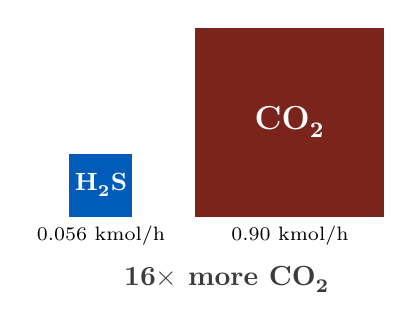
\begin{tikzpicture}[scale=0.8]
                % H2S block (small)
                \fill[MainBlue] (0,0) rectangle (1,1);
                \node[white, font=\small\bfseries] at (0.5,0.5) {\ce{H2S}};
                \node[below, font=\scriptsize] at (0.5,0) {0.056 kmol/h};

                % CO2 block (large)
                \fill[AccentC] (2,0) rectangle (5,3);
                \node[white, font=\large\bfseries] at (3.5,1.5) {\ce{CO2}};
                \node[below, font=\scriptsize] at (3.5,0) {0.90 kmol/h};

                % Label
                \node[font=\bfseries, Charcoal] at (2.5,-1) {16$\times$ more \ce{CO2}};
            \end{tikzpicture}
        \end{column}
    \end{columns}
\end{frame}

% ============================================
% SLIDE 5: Kinetic Fundamentals
% ============================================
\begin{frame}{Kinetic Fundamentals}
    \begin{columns}[T]
        \begin{column}{0.5\textwidth}
            \textbf{Reaction Rate Constants}

            \vspace{0.5em}
            \begin{tabular}{@{}lc@{}}
                \toprule
                \textbf{Reaction} & \textbf{$k$ (L/mol·s)} \\
                \midrule
                \ce{H2S + OH^-} & $\sim$10$^{10}$ \\
                \ce{CO2 + OH^-} & $\sim$10$^{3-4}$ \\
                \midrule
                \textbf{Ratio} & \textbf{$\sim$10$^6$} \\
                \bottomrule
            \end{tabular}

            \vspace{1em}
            \textbf{Damköhler Framework}
            \begin{equation*}
                \text{Da} = k \cdot C_{\ce{OH}} \cdot \tau
            \end{equation*}

            \begin{itemize}
                \item Da $\gg$ 1: reaction completes
                \item Da $\ll$ 1: reaction negligible
            \end{itemize}
        \end{column}
        \begin{column}{0.5\textwidth}
            \textbf{The Selectivity Window}

            \vspace{0.5em}
            At contact time $\tau$ = 50--100 ms:

            \vspace{0.5em}
            \begin{tabular}{@{}lcc@{}}
                \toprule
                & \textbf{Da} & \textbf{Conversion} \\
                \midrule
                \ce{H2S} & $\gg$ 1 & $\sim$100\% \\
                \ce{CO2} & $\ll$ 1 & $\sim$5\% \\
                \bottomrule
            \end{tabular}

            \vspace{1em}
            \success{Exploit kinetic difference via short contact time}
        \end{column}
    \end{columns}
\end{frame}

% ============================================
% SLIDE 6: Selectivity Window
% ============================================
\begin{frame}{Selectivity Window}
    \centering
    \resizebox{0.85\textwidth}{!}{%
        % Selectivity kinetics embedded directly
        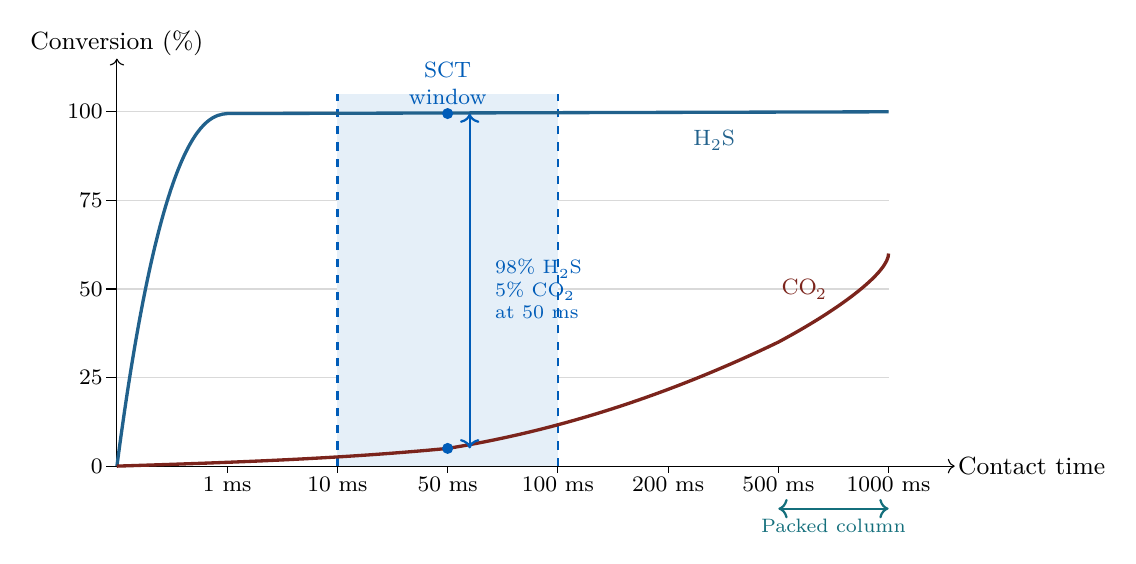
\begin{tikzpicture}[
            x=2.8cm, y=4.5cm,
            font=\small,
            every node/.style={inner sep=1pt},
        ]
          % Grid and axes
          \draw[->] (0,0) -- (3.8,0) node[right] {Contact time};
          \draw[->] (0,0) -- (0,1.15) node[above] {Conversion (\%)};

          % X-axis labels
          \foreach \x/\lab in {0.5/1, 1.0/10, 1.5/50, 2.0/100, 2.5/200, 3.0/500, 3.5/1000}
            \draw (\x,0) -- (\x,-0.02) node[below,font=\footnotesize] {\lab~ms};

          % Y-axis labels
          \foreach \y/\lab in {0/0, 0.25/25, 0.5/50, 0.75/75, 1.0/100}
            \draw (0,\y) -- (-0.05,\y) node[left,font=\footnotesize] {\lab};

          % Light grid
          \draw[gray!30, thin] (0,0.25) -- (3.5,0.25);
          \draw[gray!30, thin] (0,0.5) -- (3.5,0.5);
          \draw[gray!30, thin] (0,0.75) -- (3.5,0.75);
          \draw[gray!30, thin] (0,1.0) -- (3.5,1.0);

          % Selectivity window shading
          \fill[MainBlue!10] (1.0,0) rectangle (2.0,1.05);
          \draw[MainBlue, dashed, thick] (1.0,0) -- (1.0,1.05);
          \draw[MainBlue, dashed, thick] (2.0,0) -- (2.0,1.05);
          \node[MainBlue, font=\footnotesize, align=center] at (1.5,1.08) {SCT\\window};

          % H2S curve
          \draw[AccentA, very thick]
            (0,0)
            .. controls (0.2,0.95) and (0.4,0.99) .. (0.5,0.995)
            -- (3.5,1.0);
          \node[AccentA, anchor=west, font=\footnotesize] at (2.6,0.92) {H$_2$S};

          % CO2 curve
          \draw[AccentC, very thick]
            (0,0)
            .. controls (0.5,0.01) and (1.0,0.02) .. (1.5,0.05)
            .. controls (2.0,0.10) and (2.5,0.20) .. (3.0,0.35)
            .. controls (3.3,0.45) and (3.5,0.55) .. (3.5,0.60);
          \node[AccentC, anchor=west, font=\footnotesize] at (3.0,0.50) {CO$_2$};

          % Marker at 50ms
          \fill[MainBlue] (1.5,0.995) circle (2pt);
          \fill[MainBlue] (1.5,0.05) circle (2pt);

          % Annotation arrows
          \draw[<->, MainBlue, thick] (1.6,0.05) -- (1.6,0.995);
          \node[MainBlue, anchor=west, font=\scriptsize, align=left] at (1.7,0.5) {98\% H$_2$S\\5\% CO$_2$\\at 50~ms};

          % Packed column regime
          \draw[AccentB, thick, <->] (3.0,-0.12) -- (3.5,-0.12);
          \node[AccentB, anchor=north, font=\scriptsize] at (3.25,-0.14) {Packed column};
        \end{tikzpicture}
    }
\end{frame}

% ============================================
% SLIDE 7: Technology Comparison
% ============================================
\begin{frame}{Technology Comparison}
    \centering
    \small
    \begin{tabular}{@{}lccc@{}}
        \toprule
        \textbf{Parameter} & \textbf{Packed Column} & \textbf{SCT Mixer} & \textbf{Advantage} \\
        \midrule
        Equipment size & 0.75 m $\times$ 5.5 m & 0.3 m $\times$ 1.5 m & SCT \\
        Contact time & 5--15 s & 50--200 ms & SCT \\
        \addlinespace
        \ce{H2S} removal & 97.5\% & $>$98\% & Equal \\
        \ce{CO2} absorption & 50--80\% & 2--10\% & \textbf{SCT} \\
        \addlinespace
        NaOH consumption & 418 ton/yr & 46 ton/yr & \textbf{SCT (9$\times$)} \\
        NaOH cost & \$209k/yr & \$23k/yr & \textbf{SCT} \\
        \addlinespace
        Technology maturity & Established & Emerging & Packed \\
        Control complexity & Standard & pH-critical & Packed \\
        \bottomrule
    \end{tabular}
\end{frame}

% ============================================
% SLIDE 8: Operating Cost Impact
% ============================================
\begin{frame}{Operating Cost Impact}
    \centering
    \resizebox{0.9\textwidth}{!}{%
        % Cost Comparison Bar Chart - NaOH Annual Cost
% For use in Beamer presentation
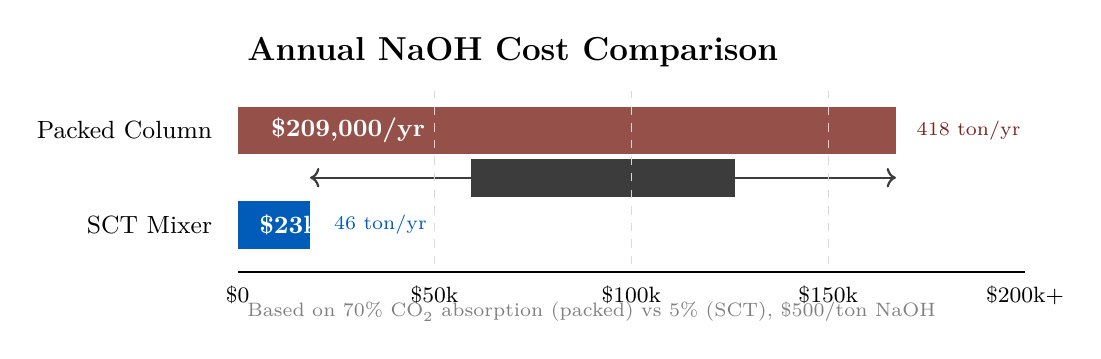
\begin{tikzpicture}[
    font=\small,
    bar/.style={minimum height=0.8cm, anchor=west},
]
    % Title
    \node[font=\large\bfseries, anchor=west] at (0,3.2) {Annual NaOH Cost Comparison};

    % Y-axis labels
    \node[anchor=east, font=\small] at (-0.2,2.2) {Packed Column};
    \node[anchor=east, font=\small] at (-0.2,1.0) {SCT Mixer};

    % Packed Column bar (AccentC - red/brown)
    \fill[AccentC!80] (0,1.9) rectangle (8.36,2.5);
    \node[anchor=west, font=\small\bfseries, white] at (0.3,2.2) {\$209,000/yr};
    \node[anchor=west, font=\scriptsize, AccentC] at (8.5,2.2) {418 ton/yr};

    % SCT bar (MainBlue)
    \fill[MainBlue] (0,0.7) rectangle (0.92,1.3);
    \node[anchor=west, font=\small\bfseries, white] at (0.15,1.0) {\$23k};
    \node[anchor=west, font=\scriptsize, MainBlue] at (1.1,1.0) {46 ton/yr};

    % X-axis
    \draw[thick] (0,0.4) -- (10,0.4);
    \foreach \x/\lab in {0/\$0, 2.5/\$50k, 5/\$100k, 7.5/\$150k, 10/\$200k+}
        \node[anchor=north, font=\footnotesize] at (\x,0.35) {\lab};

    % Annotation: cost difference
    \draw[<->, thick, Charcoal] (8.36,1.6) -- (0.92,1.6);
    \node[fill=white, font=\bfseries, Charcoal] at (4.64,1.6) {9$\times$ cost reduction};

    % Grid lines (subtle)
    \foreach \x in {2.5,5,7.5} {
        \draw[gray!30, dashed] (\x,0.5) -- (\x,2.7);
    }

    % Legend note
    \node[anchor=west, font=\scriptsize, gray] at (0,-0.1) {Based on 70\% CO$_2$ absorption (packed) vs 5\% (SCT), \$500/ton NaOH};

\end{tikzpicture}

    }
\end{frame}

% ============================================
% SLIDE 9: Economic Performance
% ============================================
\begin{frame}{Economic Performance}
    \begin{columns}[c]
        \begin{column}{0.45\textwidth}
            \textbf{Key Indicators}

            \vspace{0.5em}
            \small
            \begin{tabular}{@{}lcc@{}}
                \toprule
                & \textbf{Packed} & \textbf{SCT} \\
                \midrule
                TIC & \$2.53M & \$1.78M \\
                Net benefit & \$211k/yr & \$417k/yr \\
                Payback & 12.0 yr & 4.3 yr \\
                \textbf{IRR} & \warning{5.3\%} & \success{22.8\%} \\
                NPV & --\$87k & +\$1.06M \\
                \bottomrule
            \end{tabular}

            \vspace{1em}
            \textbf{15\% hurdle rate}
        \end{column}
        \begin{column}{0.55\textwidth}
            \centering
            \resizebox{\textwidth}{!}{%
                % Tornado diagram embedded directly
                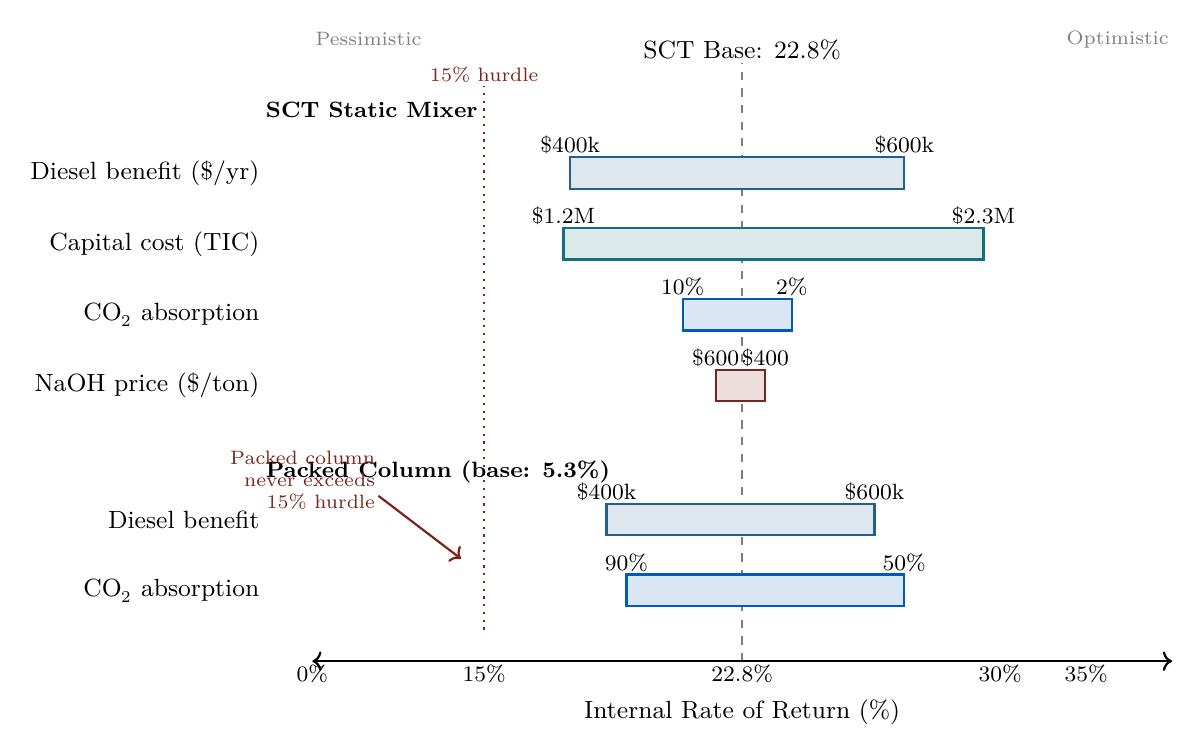
\begin{tikzpicture}[
                    x=0.42cm, y=1cm,
                    font=\small,
                    every node/.style={inner sep=1pt},
                ]
                  \def\xLabel{-14.5}
                  \def\barH{0.40}

                  % Base line (22.8% IRR for SCT base case)
                  \draw[thick,dashed,gray] (0,0.2) -- (0,7.8);
                  \node[above,font=\small] at (0,7.8) {SCT Base: 22.8\%};

                  % Hurdle rate line at 15%
                  \draw[thick,dotted,AccentC] (-7.8,0.6) -- (-7.8,7.5);
                  \node[AccentC,font=\scriptsize,anchor=south] at (-7.8,7.5) {15\% hurdle};

                  % ---- SCT Technology (top section) ----
                  \node[font=\footnotesize\bfseries,anchor=west] at (\xLabel,7.2) {SCT Static Mixer};

                  % Row 1: Diesel benefit
                  \fill[AccentA!15] (-5.2,6.2) rectangle (4.9,6.2+\barH);
                  \draw[thick,AccentA] (-5.2,6.2) rectangle (4.9,6.2+\barH);
                  \node[anchor=east] at (\xLabel,6.2+0.5*\barH) {Diesel benefit (\$/yr)};
                  \node[anchor=south, font=\footnotesize] at (-5.2,6.2+\barH) {\$400k};
                  \node[anchor=south, font=\footnotesize] at (4.9, 6.2+\barH) {\$600k};

                  % Row 2: Capital cost
                  \fill[AccentB!15] (-5.4,5.3) rectangle (7.3,5.3+\barH);
                  \draw[thick,AccentB] (-5.4,5.3) rectangle (7.3,5.3+\barH);
                  \node[anchor=east] at (\xLabel,5.3+0.5*\barH) {Capital cost (TIC)};
                  \node[anchor=south, font=\footnotesize] at (-5.4,5.3+\barH) {\$1.2M};
                  \node[anchor=south, font=\footnotesize] at (7.3, 5.3+\barH) {\$2.3M};

                  % Row 3: CO2 absorption
                  \fill[MainBlue!15] (-1.8,4.4) rectangle (1.5,4.4+\barH);
                  \draw[thick,MainBlue] (-1.8,4.4) rectangle (1.5,4.4+\barH);
                  \node[anchor=east] at (\xLabel,4.4+0.5*\barH) {CO$_2$ absorption};
                  \node[anchor=south, font=\footnotesize] at (-1.8,4.4+\barH) {10\%};
                  \node[anchor=south, font=\footnotesize] at (1.5, 4.4+\barH) {2\%};

                  % Row 4: NaOH price
                  \fill[AccentC!15] (-0.8,3.5) rectangle (0.7,3.5+\barH);
                  \draw[thick,AccentC] (-0.8,3.5) rectangle (0.7,3.5+\barH);
                  \node[anchor=east] at (\xLabel,3.5+0.5*\barH) {NaOH price (\$/ton)};
                  \node[anchor=south, font=\footnotesize] at (-0.8,3.5+\barH) {\$600};
                  \node[anchor=south, font=\footnotesize] at (0.7, 3.5+\barH) {\$400};

                  % ---- Packed Column (bottom section) ----
                  \node[font=\footnotesize\bfseries,anchor=west] at (\xLabel,2.6) {Packed Column (base: 5.3\%)};

                  % Row 5: Diesel benefit (packed)
                  \fill[AccentA!15] (-4.1,1.8) rectangle (4.0,1.8+\barH);
                  \draw[thick,AccentA] (-4.1,1.8) rectangle (4.0,1.8+\barH);
                  \node[anchor=east] at (\xLabel,1.8+0.5*\barH) {Diesel benefit};
                  \node[anchor=south, font=\footnotesize] at (-4.1,1.8+\barH) {\$400k};
                  \node[anchor=south, font=\footnotesize] at (4.0, 1.8+\barH) {\$600k};

                  % Row 6: CO2 absorption (packed)
                  \fill[MainBlue!15] (-3.5,0.9) rectangle (4.9,0.9+\barH);
                  \draw[thick,MainBlue] (-3.5,0.9) rectangle (4.9,0.9+\barH);
                  \node[anchor=east] at (\xLabel,0.9+0.5*\barH) {CO$_2$ absorption};
                  \node[anchor=south, font=\footnotesize] at (-3.5,0.9+\barH) {90\%};
                  \node[anchor=south, font=\footnotesize] at (4.9, 0.9+\barH) {50\%};

                  % X-axis
                  \draw[<->,thick] (-13,0.2) -- (13,0.2);
                  \foreach \x/\lab in {-13/0, -7.8/15, 0/22.8, 7.8/30, 10.4/35}
                    \node[below,font=\footnotesize] at (\x,0.2) {\lab\%};

                  \node[below] at (0,-0.25) {Internal Rate of Return (\%)};

                  % Annotations
                  \node[anchor=west,font=\scriptsize,gray] at (-13,8.1) {Pessimistic};
                  \node[anchor=east,font=\scriptsize,gray] at (13,8.1) {Optimistic};

                  % Highlight: packed column never exceeds hurdle
                  \draw[AccentC, thick, ->] (-11,2.3) -- (-8.5,1.5);
                  \node[AccentC, font=\scriptsize, anchor=east, align=right] at (-11,2.5) {Packed column\\never exceeds\\15\% hurdle};
                \end{tikzpicture}
            }
        \end{column}
    \end{columns}
\end{frame}

% ============================================
% SLIDE 10: Process Configuration
% ============================================
\begin{frame}{Process Configuration}
    \centering
    \includegraphics[width=0.85\textwidth]{BFD - Caustic Scrubbing.png}
\end{frame}

% ============================================
% SLIDE 11: Control & Safety
% ============================================
\begin{frame}{Control \& Safety}
    \centering
    \resizebox{0.9\textwidth}{!}{%
        % Control loops embedded directly
        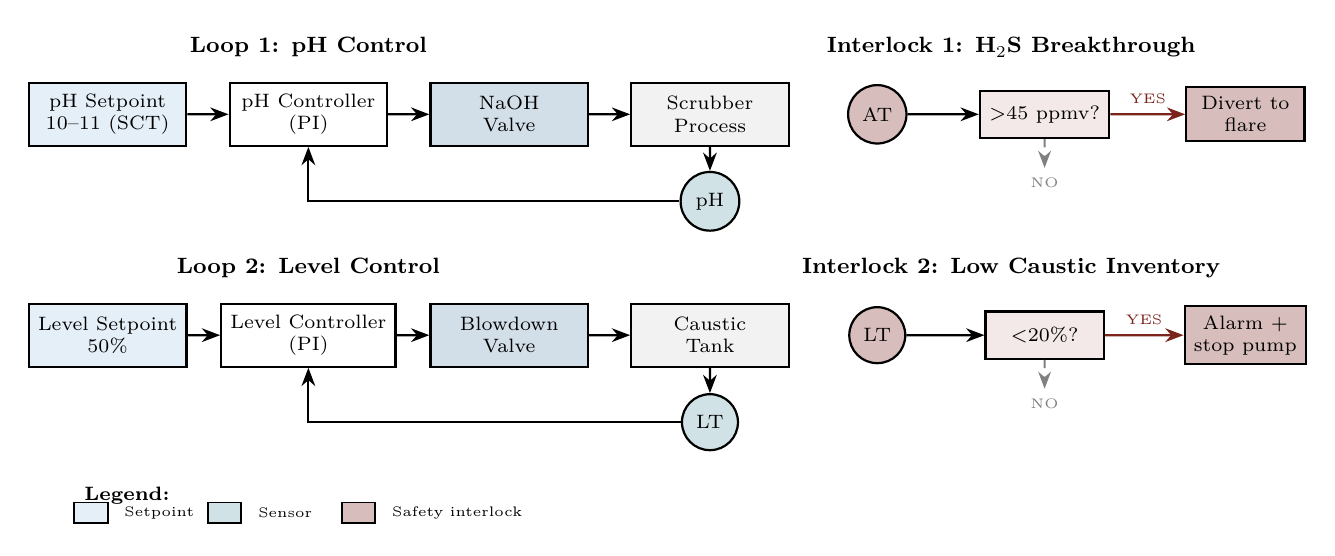
\begin{tikzpicture}[
            scale=0.85,
            font=\small,
            >=Stealth,
            line width=0.7pt,
            block/.style={rectangle, draw, thick, minimum width=2cm, minimum height=0.8cm, align=center, font=\scriptsize},
            smallblock/.style={rectangle, draw, thick, minimum width=1.5cm, minimum height=0.6cm, align=center, font=\scriptsize},
            sensor/.style={circle, draw, thick, minimum size=0.6cm, font=\scriptsize},
        ]

        % ===== CONTROL LOOP 1: pH Control =====
        \node[font=\footnotesize\bfseries] at (0,6.5) {Loop 1: pH Control};

        \node[block, fill=MainBlue!10] (sp1) at (-3,5.5) {pH Setpoint\\10--11 (SCT)};
        \node[block, fill=white] (pic) at (0,5.5) {pH Controller\\(PI)};
        \node[block, fill=AccentA!20] (valve1) at (3,5.5) {NaOH\\Valve};
        \node[block, fill=gray!10] (proc1) at (6,5.5) {Scrubber\\Process};
        \node[sensor, fill=AccentB!20] (ph) at (6,4.2) {pH};

        \draw[->, thick] (sp1) -- (pic);
        \draw[->, thick] (pic) -- (valve1);
        \draw[->, thick] (valve1) -- (proc1);
        \draw[->, thick] (proc1) -- (ph);
        \draw[->, thick] (ph) -| (0,4.2) -- (pic);

        % ===== CONTROL LOOP 2: Level Control =====
        \node[font=\footnotesize\bfseries] at (0,3.2) {Loop 2: Level Control};

        \node[block, fill=MainBlue!10] (sp2) at (-3,2.2) {Level Setpoint\\50\%};
        \node[block, fill=white] (lic) at (0,2.2) {Level Controller\\(PI)};
        \node[block, fill=AccentA!20] (valve2) at (3,2.2) {Blowdown\\Valve};
        \node[block, fill=gray!10] (proc2) at (6,2.2) {Caustic\\Tank};
        \node[sensor, fill=AccentB!20] (lt) at (6,0.9) {LT};

        \draw[->, thick] (sp2) -- (lic);
        \draw[->, thick] (lic) -- (valve2);
        \draw[->, thick] (valve2) -- (proc2);
        \draw[->, thick] (proc2) -- (lt);
        \draw[->, thick] (lt) -| (0,0.9) -- (lic);

        % ===== INTERLOCK 1: H2S Breakthrough =====
        \node[font=\footnotesize\bfseries] at (10.5,6.5) {Interlock 1: H$_2$S Breakthrough};

        \node[sensor, fill=AccentC!30] (at) at (8.5,5.5) {AT};
        \node[smallblock, fill=AccentC!10] (logic1) at (11,5.5) {>45 ppmv?};
        \node[smallblock, fill=AccentC!30] (action1) at (14,5.5) {Divert to\\flare};

        \draw[->, thick] (at) -- (logic1);
        \draw[->, thick, AccentC] (logic1) -- node[above, font=\tiny] {YES} (action1);
        \draw[->, dashed, gray] (logic1) -- ++(0,-0.8) node[below, font=\tiny] {NO};

        % ===== INTERLOCK 2: Low Caustic =====
        \node[font=\footnotesize\bfseries] at (10.5,3.2) {Interlock 2: Low Caustic Inventory};

        \node[sensor, fill=AccentC!30] (lt2) at (8.5,2.2) {LT};
        \node[smallblock, fill=AccentC!10] (logic2) at (11,2.2) {<20\%?};
        \node[smallblock, fill=AccentC!30] (action2) at (14,2.2) {Alarm +\\stop pump};

        \draw[->, thick] (lt2) -- (logic2);
        \draw[->, thick, AccentC] (logic2) -- node[above, font=\tiny] {YES} (action2);
        \draw[->, dashed, gray] (logic2) -- ++(0,-0.8) node[below, font=\tiny] {NO};

        % Legend
        \node[font=\scriptsize, anchor=west] at (-3.5,-0.2) {\textbf{Legend:}};
        \fill[MainBlue!10] (-3.5,-0.6) rectangle (-3.0,-0.3);
        \draw (-3.5,-0.6) rectangle (-3.0,-0.3);
        \node[font=\tiny, anchor=west] at (-2.9,-0.45) {Setpoint};
        \fill[AccentB!20] (-1.5,-0.6) rectangle (-1.0,-0.3);
        \draw (-1.5,-0.6) rectangle (-1.0,-0.3);
        \node[font=\tiny, anchor=west] at (-0.9,-0.45) {Sensor};
        \fill[AccentC!30] (0.5,-0.6) rectangle (1.0,-0.3);
        \draw (0.5,-0.6) rectangle (1.0,-0.3);
        \node[font=\tiny, anchor=west] at (1.1,-0.45) {Safety interlock};
        \end{tikzpicture}
    }
\end{frame}

% ============================================
% SLIDE 12: Recommendation & Next Steps
% ============================================
\begin{frame}{Recommendation \& Next Steps}
    \centering
    \resizebox{0.85\textwidth}{!}{%
        % Recommendation Summary - Technology Decision Visual
% For use in Beamer presentation
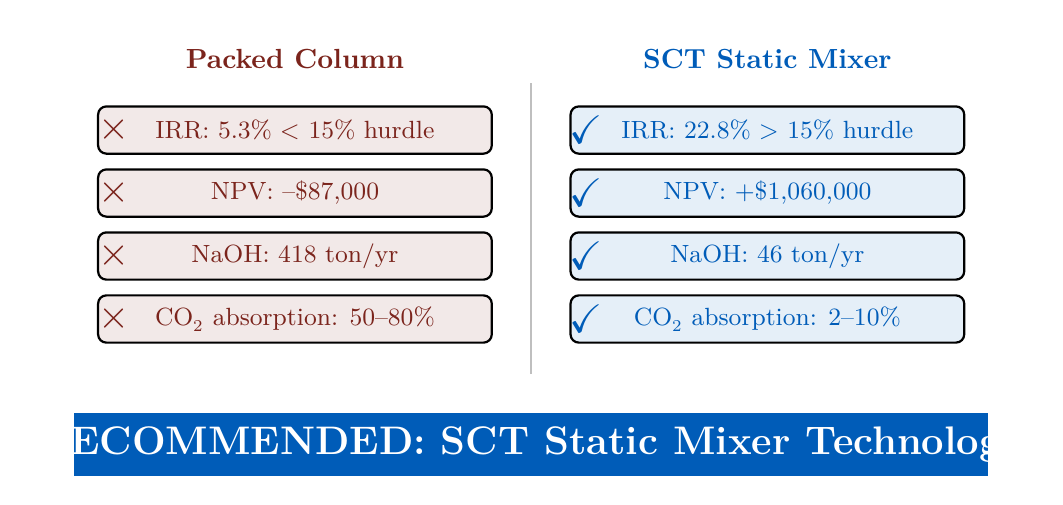
\begin{tikzpicture}[
    font=\small,
    box/.style={rectangle, draw, thick, rounded corners=3pt, minimum width=5cm, minimum height=0.6cm, align=center},
    header/.style={font=\bfseries, minimum height=0.8cm},
]
    % Column headers
    \node[header, AccentC] at (2.5,4.5) {Packed Column};
    \node[header, MainBlue] at (8.5,4.5) {SCT Static Mixer};

    % Packed Column cons (left)
    \node[box, fill=AccentC!10, text=AccentC] at (2.5,3.6) {IRR: 5.3\% $<$ 15\% hurdle};
    \node[box, fill=AccentC!10, text=AccentC] at (2.5,2.8) {NPV: --\$87,000};
    \node[box, fill=AccentC!10, text=AccentC] at (2.5,2.0) {NaOH: 418 ton/yr};
    \node[box, fill=AccentC!10, text=AccentC] at (2.5,1.2) {CO$_2$ absorption: 50--80\%};

    % SCT pros (right)
    \node[box, fill=MainBlue!10, text=MainBlue] at (8.5,3.6) {IRR: 22.8\% $>$ 15\% hurdle};
    \node[box, fill=MainBlue!10, text=MainBlue] at (8.5,2.8) {NPV: +\$1,060,000};
    \node[box, fill=MainBlue!10, text=MainBlue] at (8.5,2.0) {NaOH: 46 ton/yr};
    \node[box, fill=MainBlue!10, text=MainBlue] at (8.5,1.2) {CO$_2$ absorption: 2--10\%};

    % X marks for Packed
    \foreach \y in {3.6, 2.8, 2.0, 1.2} {
        \node[AccentC, font=\Large\bfseries] at (0.2,\y) {$\times$};
    }

    % Checkmarks for SCT
    \foreach \y in {3.6, 2.8, 2.0, 1.2} {
        \node[MainBlue, font=\Large\bfseries] at (6.2,\y) {$\checkmark$};
    }

    % Divider line
    \draw[thick, gray!50] (5.5,0.5) -- (5.5,4.2);

    % Recommendation banner
    \fill[MainBlue] (-0.3,0) rectangle (11.3,-0.8);
    \node[white, font=\Large\bfseries] at (5.5,-0.4) {RECOMMENDED: SCT Static Mixer Technology};

    % % Next steps section
    % \node[font=\bfseries, anchor=west] at (-0.3,-1.4) {Next Steps:};

    % \node[anchor=west, font=\small] at (0,-1.9) {1. Issue RFQ to SCT vendors (Merichem, Trimeric, Koch-Glitsch)};
    % \node[anchor=west, font=\small] at (0,-2.4) {2. Validate diesel displacement via operational data};
    % \node[anchor=west, font=\small] at (0,-2.9) {3. Conduct HAZID workshop};
    % \node[anchor=west, font=\small] at (0,-3.4) {4. Proceed to FEED study};

\end{tikzpicture}

    }
\end{frame}

% ============================================
% BACKUP SLIDES
% ============================================
\appendix

\begin{frame}{Backup: Packed Column Schematic}
    \centering
    \resizebox{0.5\textwidth}{!}{%
        % Packed column embedded directly
        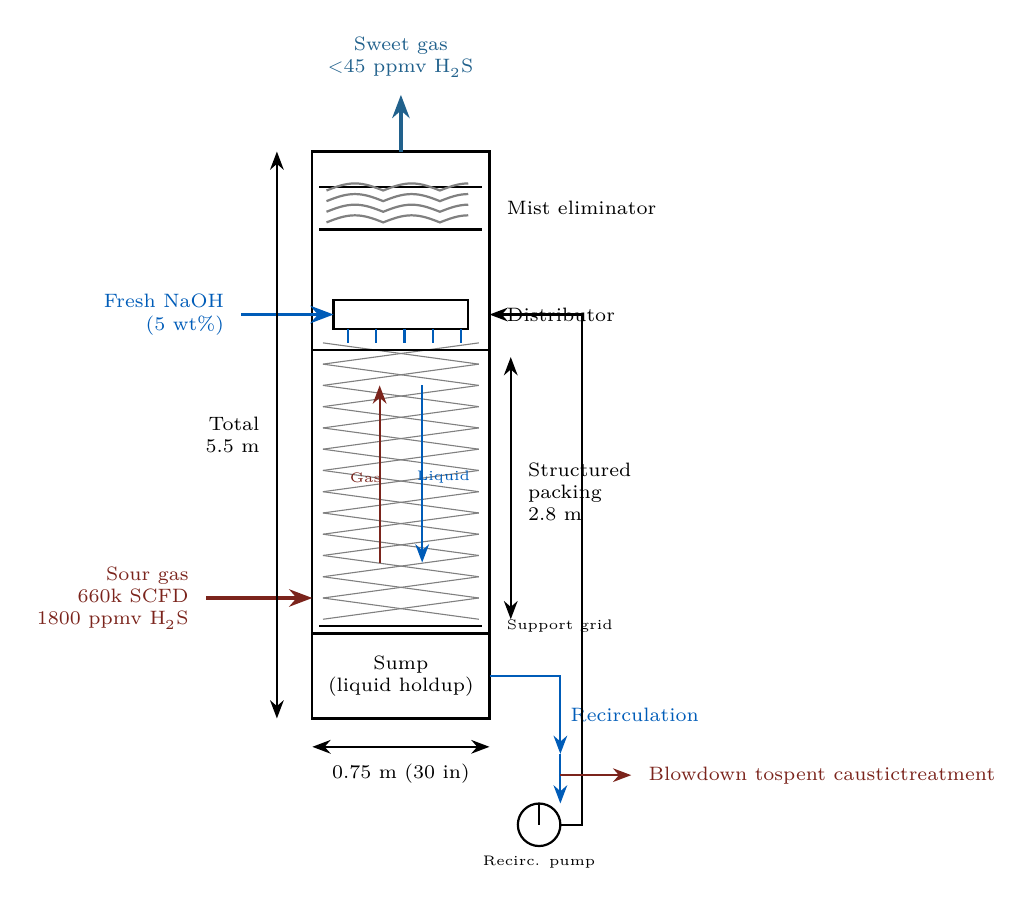
\begin{tikzpicture}[
            scale=0.9,
            font=\small,
            >=Stealth,
            line width=0.8pt,
        ]

        % Column vessel outline
        \def\colW{2.5}
        \def\colH{8.0}
        \def\sumpH{1.2}
        \def\packH{4.0}
        \def\distH{0.4}
        \def\mistH{0.6}

        % Main vessel
        \draw[thick] (0,0) -- (0,\colH) -- (\colW,\colH) -- (\colW,0) -- cycle;

        % Sump section
        \draw[thick] (0,\sumpH) -- (\colW,\sumpH);
        \node[font=\scriptsize, align=center] at (\colW/2, \sumpH/2) {Sump\\(liquid holdup)};

        % Packing support
        \draw[thick] (0.1,\sumpH+0.1) -- (\colW-0.1,\sumpH+0.1);
        \node[font=\tiny, anchor=west] at (\colW+0.1, \sumpH+0.1) {Support grid};

        % Packing section (hatched)
        \foreach \y in {0,0.3,...,3.9} {
            \draw[gray, thin] (0.15,\sumpH+0.2+\y) -- (\colW-0.15,\sumpH+0.5+\y);
            \draw[gray, thin] (0.15,\sumpH+0.5+\y) -- (\colW-0.15,\sumpH+0.2+\y);
        }
        \draw[thick] (0,\sumpH+\packH) -- (\colW,\sumpH+\packH);

        % Packing label
        \draw[<->, thick] (\colW+0.3, \sumpH+0.2) -- (\colW+0.3, \sumpH+\packH-0.1);
        \node[font=\scriptsize, anchor=west, align=left] at (\colW+0.4, \sumpH+\packH/2) {Structured\\packing\\2.8~m};

        % Liquid distributor
        \draw[thick, fill=white] (0.3,\sumpH+\packH+0.3) rectangle (\colW-0.3,\sumpH+\packH+0.3+\distH);
        \foreach \x in {0.5,0.9,1.3,1.7,2.1} {
            \draw[MainBlue, thick] (\x,\sumpH+\packH+0.3) -- (\x,\sumpH+\packH+0.1);
        }
        \node[font=\scriptsize, anchor=west] at (\colW+0.1, \sumpH+\packH+0.5) {Distributor};

        % Mist eliminator
        \draw[thick] (0.1,\colH-\mistH-0.5) -- (\colW-0.1,\colH-\mistH-0.5);
        \draw[thick] (0.1,\colH-0.5) -- (\colW-0.1,\colH-0.5);
        \foreach \y in {0,0.15,...,0.55} {
            \draw[gray] (0.2,\colH-\mistH-0.4+\y) sin (0.6,\colH-\mistH-0.3+\y) cos (1.0,\colH-\mistH-0.4+\y) sin (1.4,\colH-\mistH-0.3+\y) cos (1.8,\colH-\mistH-0.4+\y) sin (2.2,\colH-\mistH-0.3+\y);
        }
        \node[font=\scriptsize, anchor=west] at (\colW+0.1, \colH-\mistH/2-0.5) {Mist eliminator};

        % Gas inlet (bottom)
        \draw[AccentC, very thick, ->] (-1.5,\sumpH+0.5) -- (0,\sumpH+0.5);
        \node[AccentC, font=\scriptsize, anchor=east, align=right] at (-1.6,\sumpH+0.5) {Sour gas\\660k SCFD\\1800 ppmv H$_2$S};

        % Gas outlet (top)
        \draw[AccentA, very thick, ->] (\colW/2,\colH) -- (\colW/2,\colH+0.8);
        \node[AccentA, font=\scriptsize, anchor=south, align=center] at (\colW/2,\colH+0.9) {Sweet gas\\$<$45 ppmv H$_2$S};

        % Liquid inlet (top)
        \draw[MainBlue, very thick, ->] (-1.0,\sumpH+\packH+0.5) -- (0.3,\sumpH+\packH+0.5);
        \node[MainBlue, font=\scriptsize, anchor=east, align=right] at (-1.1,\sumpH+\packH+0.5) {Fresh NaOH\\(5 wt\%)};

        % Liquid outlet / recirculation
        \draw[MainBlue, thick, ->] (\colW,\sumpH/2) -- (\colW+1.0,\sumpH/2) -- (\colW+1.0,-0.5) node[midway, anchor=west, font=\scriptsize] {Recirculation};
        \draw[MainBlue, thick, ->] (\colW+1.0,-0.5) -- (\colW+1.0,-1.2);

        % Pump symbol
        \draw[thick] (\colW+0.7,-1.5) circle (0.3);
        \draw[thick] (\colW+0.7,-1.2) -- (\colW+0.7,-1.5);
        \draw[thick, ->] (\colW+1.0,-1.5) -- (\colW+1.3,-1.5) -- (\colW+1.3,\sumpH+\packH+0.5) -- (\colW,\sumpH+\packH+0.5);
        \node[font=\tiny, anchor=north] at (\colW+0.7,-1.8) {Recirc. pump};

        % Blowdown
        \draw[AccentC, thick, ->] (\colW+1.0,-0.8) -- (\colW+2.0,-0.8);
        \node[AccentC, font=\scriptsize, anchor=west] at (\colW+2.1,-0.8) {Blowdown to\\spent caustic\\treatment};

        % Dimension: column diameter
        \draw[<->, thick] (0,-0.4) -- (\colW,-0.4);
        \node[font=\scriptsize, anchor=north] at (\colW/2,-0.5) {0.75~m (30~in)};

        % Dimension: total height
        \draw[<->, thick] (-0.5,0) -- (-0.5,\colH);
        \node[font=\scriptsize, anchor=east, align=right] at (-0.6,\colH/2) {Total\\5.5~m};

        % Flow direction arrows inside column
        \draw[AccentC, ->, thick] (\colW/2-0.3,\sumpH+1.0) -- (\colW/2-0.3,\sumpH+3.5);
        \draw[MainBlue, ->, thick] (\colW/2+0.3,\sumpH+3.5) -- (\colW/2+0.3,\sumpH+1.0);
        \node[font=\tiny, AccentC] at (\colW/2-0.5,\sumpH+2.2) {Gas};
        \node[font=\tiny, MainBlue] at (\colW/2+0.6,\sumpH+2.2) {Liquid};
        \end{tikzpicture}
    }
\end{frame}

\begin{frame}{Backup: Capital Cost Breakdown}
    \centering
    \small
    \begin{tabular}{@{}lcc@{}}
        \toprule
        \textbf{Cost Element} & \textbf{Packed Column} & \textbf{SCT System} \\
        \midrule
        Scrubber/contactor & \$450,000 & \$180,000 \\
        Caustic storage \& dosing & \$150,000 & \$120,000 \\
        Spent caustic treatment (MBBR) & \$350,000 & \$300,000 \\
        Instrumentation \& controls & \$180,000 & \$200,000 \\
        Piping \& bulks & \$220,000 & \$150,000 \\
        \midrule
        \textbf{Direct costs} & \textbf{\$1,350,000} & \textbf{\$950,000} \\
        \midrule
        Engineering (15\%) & \$203,000 & \$143,000 \\
        Installation (35\%) & \$473,000 & \$333,000 \\
        Contingency (25\%) & \$507,000 & \$357,000 \\
        \midrule
        \textbf{Total Installed Cost} & \textbf{\$2,530,000} & \textbf{\$1,780,000} \\
        \bottomrule
    \end{tabular}
\end{frame}

\begin{frame}{Backup: Sensitivity Analysis}
    \centering
    \small
    \begin{tabular}{@{}lccccc@{}}
        \toprule
        \textbf{Parameter} & \textbf{Range} & \multicolumn{2}{c}{\textbf{Packed Column}} & \multicolumn{2}{c}{\textbf{SCT System}} \\
        & & Low & High & Low & High \\
        \midrule
        \ce{CO2} absorption & 50--90\% / 2--10\% & 10.2\% & 1.8\% & 24.3\% & 21.0\% \\
        Capital cost & $\pm$30\% & 9.5\% & 2.3\% & 30.1\% & 17.4\% \\
        Diesel benefit & \$400k--\$600k/yr & 1.2\% & 9.3\% & 17.6\% & 27.7\% \\
        NaOH price & \$400--\$600/ton & 6.8\% & 3.7\% & 23.5\% & 22.0\% \\
        \bottomrule
    \end{tabular}

    \vspace{1em}
    \textbf{Key Finding:} SCT exceeds 15\% hurdle in all scenarios; Packed Column never reaches hurdle.
\end{frame}

\begin{frame}{Backup: Spent Caustic Treatment}
    \begin{columns}[T]
        \begin{column}{0.5\textwidth}
            \textbf{MBBR Design Basis}

            \vspace{0.5em}
            \begin{tabular}{@{}lc@{}}
                \toprule
                \textbf{Parameter} & \textbf{Value} \\
                \midrule
                Sulfide load & 43 kg S/day \\
                Reactor volume & 50 m$^3$ \\
                Media fill & 40\% \\
                Media type & K3 carriers \\
                HRT & 8--16 hours \\
                \bottomrule
            \end{tabular}
        \end{column}
        \begin{column}{0.5\textwidth}
            \textbf{Biological Oxidation}

            \vspace{0.5em}
            Partial oxidation (preferred):
            \begin{equation*}
                \ce{HS^- + 0.5 O2 -> S^0 + OH^-}
            \end{equation*}

            \vspace{0.5em}
            Benefits:
            \begin{itemize}
                \item Recoverable elemental sulfur
                \item Alkalinity regeneration (40--60\%)
                \item Lower operating cost vs chemical oxidation
            \end{itemize}
        \end{column}
    \end{columns}
\end{frame}

\end{document}
